\section{Esercitazione 7}
\title{LEZIONE 17 8/04/2020}\newline
\textbf{link} \href{https://web.microsoftstream.com/video/5d3f8bd1-ee8b-420b-802f-14dfed0bd278?list=user&userId=faa91214-a6f5-40d7-8875-253fd49b8ce1}{clicca qui}\newline
\newline
Appunti del prof con annotazioni \url{../pdf/FdA-L17-2020.04.08.pdf}\newline
Contenuto:
\begin{itemize}
    \item Diagramma polare;
    \item Effetto di un ritardo sulla risposta in frequenza e sulle sue rappresentazioni (Bode e diagramma polare);
\end{itemize}
\subsection{Diagrammi polari}
A differenza dei diagrammi di Bode, i diagrammi polari non hanno metodi comodi per tracciarne l'andamento. Possiamo però comprenderne l'andamento tramite un'analisi del comportamento asintotico per $\omega \rightarrow 0^+$ e per $\omega \rightarrow  \infty$ e tramite un'analisi dell'aspetto qualitativo.\newline
\newline
Quindi studiamo la generica funzione di trasferimento $G(s)$ nella classica forma con cui la analizzeremmo per Bode.
\begin{itemize}
    \item Per prima cosa analiziamo il comportamento per $\omega = 0$ (se $G$ è definita in $0$, altrimenti si studia il comportamento per $\omega \rightarrow  0^+$):
    \begin{itemize}
        \item Se $g=0$, allora $G(0) = \mu$ e quindi il diagramma polare parte dall'asse reale, a sinistra dell'origine se $\mu<0$ o a destra dell'origine se $\mu>0$ o dall'origine se $\mu=0$;
        \item Se $g>0$ si dice che il diagramma polare della funzione $G$ "parte all'infinito" con fase $-g \cdot 90^o$ (es. se $g=1$ la dase è $-90^o$ e quindi il diagramma di bode "parte all'infinito" dal basso). Notiamo che nel dire che "parte all'infinito" non significa che parta dall'asse, può partire da un qualunque punto.
        [immagine dagli appunti del prof]
        \begin{center}
            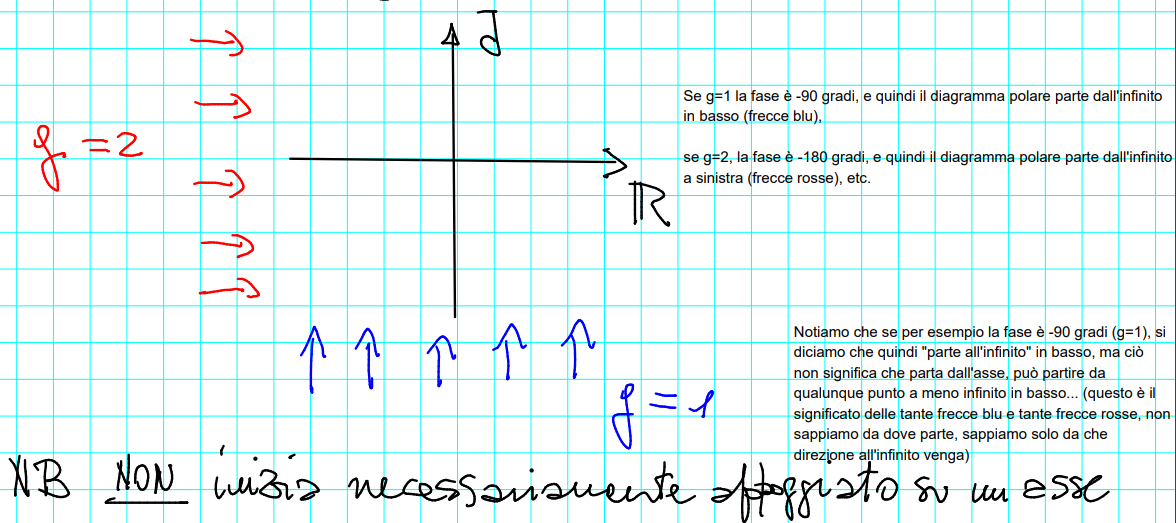
\includegraphics[height=5cm]{../lezione17/img1.PNG}
        \end{center}
    \end{itemize}
    \item Analiziamo ora il comportamento per $\omega \rightarrow  \infty$ e distinguiamo due casi:
    \begin{itemize}
        \item Numero di zeri uguale al numero di poli: Il modulo è una costante e l'argomento è un multiplo intero di $180^o$ oppure anche $0^o$ (perchè ogni polo e ogni zero ha un contributo di $90^o$ e se il numero di poli e di zeri è uguale, allora abbiamo una quantità pari di sfasamenti di $90^o$.)
        \item Numero di poli maggiore del numero di zeri: Il modulo tende a $0$ e la fase è un multiplo intero di $90^o$ oppure anche $0^o$.
    \end{itemize}
    \item Analiziamo ora l'aspetto qualitativo del diagramma polare deducendolo dal diagramma di Bode e ricordando che l'andamento del modulo rappresenta l'andamento della distanza dall'origine e che l'andamento della fase rappresetna l'andamento dell'argomento.\newline
    \newline
    Per esempio osservando l'andamento del modulo nel diagramma di Bode possiamo dedurre se il diagramma di bode si allontana dall'origine o si avvicina etc., invece osservando la fase nel diagramma di Bode possiamo dedurre in quali quadranti apparterrà il diagramma polare o con che angolo finisce o inizia etc.
    \item Analiziamo gli effetti di un ritardo applicato a una funzione di trasferimento. Prendiamo $G(s) = \frac{N(s)}{D(s)} e^{-s \tau} = G_R(s) e^{-s \tau}$, in cui $G_R(s)$ rappresenta la dianmica razionale (cioè una tipica funzione di trasferimento) e $e^{-s \tau}$ un ritardo.
    \[
        G(j \omega) = G_r(j \omega) e^{- j \omega \tau} = \begin{cases}
            |G(j \omega)| = |G_R(j \omega)|\\
            arg(G(j \omega)) = arg(G_R(j \omega)) - \omega \tau
        \end{cases}
    \]
    Notiamo che il ritardo non ha effetti sul modulo, ma solo sulla fase con il termine $- \omega \tau$ che è espresso in radianti (\textbf{oss.} Errore tipico è scordarsi di trasformare le radianti in gradi).\newline
    Quindi gli effetti del ritardo sul diagramma di Bode del modulo sono nulli, mentre sul diagramma di Bode della fase il ritardo ha un contributo lineare $- \omega \tau$, che in scala logaritmica è rappresentato da un esponenziale.\newline
    \newline
    Ai fini pratici (in esame) l'unica cosa che ci può essere richiesta è il calcolo di di una funzione di trasferimento ritardata tramite il regolo delle fasi. Per farlo studiamo la funzione di trasferimento ignorando il ritardo e alla fine di tutti i calcoli con il regolo delle fasi, ci basta sottrarre $\omega \tau$ (RADIANTI! ricordati di trasformarli in gradi). \newline
    \newline
    L'effetto grafico che si ha su un diagramma polare a causa di un ritardo è che l'intero diagramma polare viene "arrotolato su sè stesso".\newline
    [immagine dagli appunti del prof]
    \begin{center}
        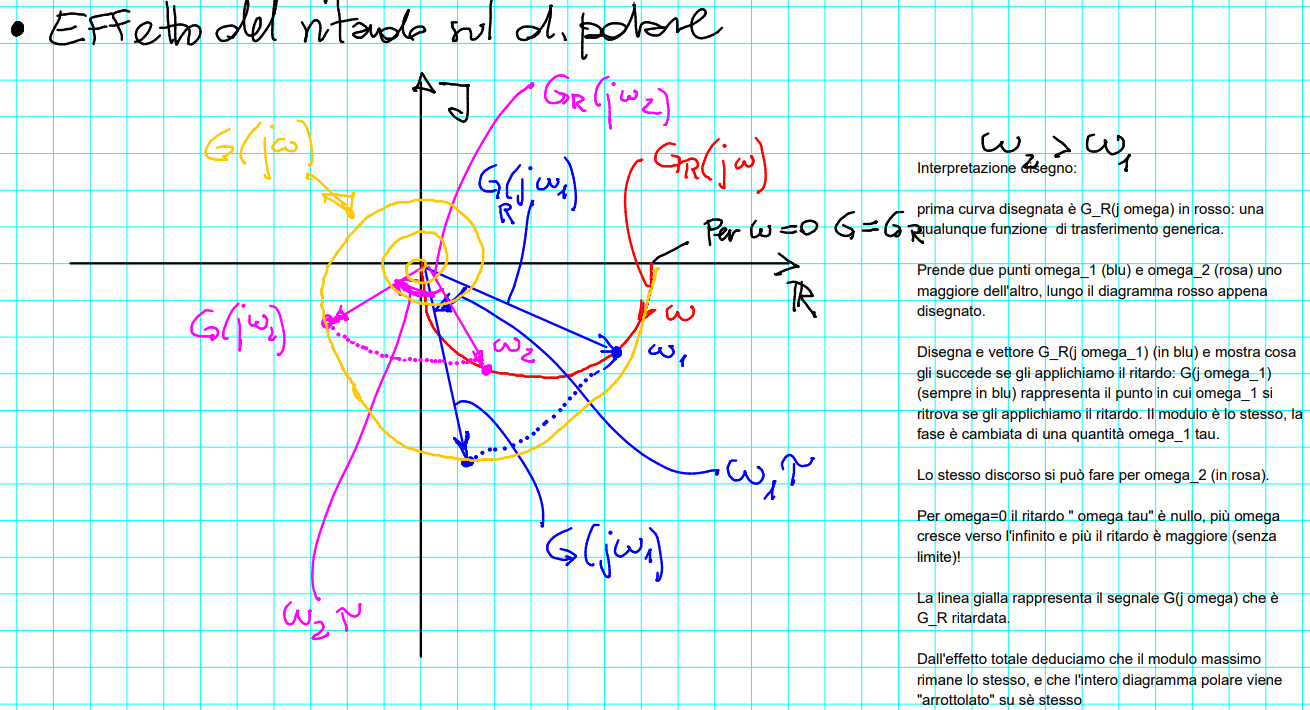
\includegraphics[height=7cm]{../lezione17/img2.PNG}
    \end{center}
    Data $G = \frac{N}{D} e^{- j \omega \tau}$ ci sono due casi possibili:
    \begin{itemize}
        \item Caso in cui il grado di $D$ sia maggiore del grado di $N$: il diagramma polare di $G$ dinisce nell'origine con fase tendente a $- \infty$, quindi il diagramma si arrotola su sè stesso come una spirale;
        \item Caso in cui il grado di $D$ sia uguale al grado di $N$: il modulo è costante e la fase tende a $- \infty$, quindi il diagramma diventa una circonferenza percorsa infinite volte.
    \end{itemize}
\end{itemize}